% sumber: doc/P4_FEED_NOTES.md, isu #308 sampai #316, komentar Brian pada isu #401 (uji coba P4 pada klaster tiga VM), services/aggregator (fire_*.go)
\chapter[MILESTONE 2: PROBLEM 4]{Milestone 2: Problem 4, Titik Api dari Satelit}

Bab ini menjawab Problem 4 Milestone 2. Fakta tentang aliran satelit diambil dari pengukuran di \texttt{doc/P4\_FEED\_NOTES.md} (profil latihan, kecepatan 60). Bukti pemulihan diambil dari uji coba Brian pada klaster tiga VM yang dicatat di isu \#401. Bagian yang belum ada buktinya ditandai.

\section{Identifikasi Persoalan}

\begin{longtable}[]{|>{\raggedright\arraybackslash}p{0.3\linewidth}|>{\raggedright\arraybackslash}p{0.3\linewidth}|>{\raggedright\arraybackslash}p{0.3\linewidth}|}
\hline
\textbf{Persoalan} & \textbf{Konsep dalam literatur} & \textbf{Wujud pada soal} \\
\hline
\endhead
Deteksi datang terlambat dan tidak berurutan & \textit{Event time} melawan \textit{processing time}, \textit{allowed lateness}, \textit{watermark} & Keterlambatan p99,9 sekitar 4 jam, maksimum 5 jam 1 menit \\
\hline
Deteksi dikirim ulang, diperbarui, atau ditarik & \textit{Idempotent consumer}, \textit{tombstone} & 6,5\% deteksi adalah kiriman ulang; ada \texttt{update} dan \texttt{retract} per kunci \\
\hline
Hanya satu koneksi aliran per kelompok & \textit{Leader election} dengan \textit{lease} & Koneksi kedua mendapat 429 dan mengusir koneksi pertama \\
\hline
Pembaca bisa mati kapan saja & Pemulihan dengan membaca ulang log dan \textit{offset} yang tersimpan & Hasil titik api harus sama dengan atau tanpa \textit{crash} \\
\hline
\end{longtable}

\section{Rancangan}

\textbf{Satu pembaca.} Hanya pemegang \textit{lease} SATELIT yang membuka aliran, karena koneksi kedua mengusir koneksi pertama dan keduanya akan saling menjatuhkan. Pembaca menyambung ulang dengan \texttt{Last-Event-ID} sesudah server menutup aliran, yang terjadi tiap 9 sampai 90 detik.

\textbf{Alur.} Pembaca SSE mengisi antrean terbatas berisi 2.048 rekaman, lalu \textit{fire engine} memprosesnya, dan hasilnya disimpan per \textit{micro-batch} setiap 500 peristiwa atau 1 detik. Urutan di tiap \textit{batch} tetap: \textit{upsert} kebakaran, parkir peristiwa yang ditolak, terbitkan dan tunggu konfirmasi \textit{broker}, baru majukan \textit{bookmark}. Bila antrean penuh, pembaca berhenti membaca dan melanjutkan dari \textit{offset} terakhir, jadi tidak ada data yang dibuang.

\textbf{Pengelompokan.} Dua deteksi terhubung bila jaraknya paling jauh 1,0 km (haversine) dan selisih waktunya paling lama 360 menit, dan hubungan ini berantai. Kebakaran adalah kumpulan deteksi yang terhubung dengan minimal dua deteksi. Deteksi dengan \textit{confidence} \texttt{l} tidak ikut. \textit{Fire engine} tidak melakukan I/O dan tidak membaca jam dinding, jadi peristiwa yang sama dengan urutan yang sama selalu menghasilkan kebakaran, nama, dan versi yang sama. Kiriman ulang dilewati, \texttt{update} mengubah \textit{confidence} atau FRP, dan \texttt{retract} bersifat final.

\textbf{Nama dan pemetaan.} Nama kebakaran diambil dari \textit{anchor}, yaitu deteksi dengan \textit{offset} terkecil. Bila dua kebakaran bergabung, \textit{anchor} yang lebih kecil menang. Nama tetap walau \textit{anchor} ditarik, jadi data terlambat atau pembacaan ulang tidak mengganti nama. Setiap kebakaran menjadi HazardEvent WILDFIRE dengan posisi titik tengah semua deteksinya dan waktu deteksi paling awal. Tingkatnya AWAS bila minimal 20 deteksi atau total FRP minimal 100 MW, SIAGA bila minimal 6 deteksi atau 30 MW, selain itu WASPADA.

\textbf{Kunci deteksi.} Deteksi dikenali dengan kunci lima \textit{field} \texttt{satellite|acq\_date|acq\_time|latitude|longitude}, dengan koordinat ditulis desimal biasa lima angka seperti kunci pada \texttt{update} dan \texttt{retract}. Kiriman ulang dengan isi sama dilewati. \texttt{retract} meninggalkan \textit{tombstone} yang menang atas kiriman ulang berikutnya.

\textbf{Jam umpan dan keterlambatan.} Jam umpan adalah nilai terbesar dari \texttt{virtual\_now} \textit{heartbeat} terakhir dan \texttt{acq} terbaru. Batas keterlambatan $L = 12$ jam, lebih dari dua kali keterlambatan terbesar yang terukur. Peristiwa yang lebih terlambat disimpan di \texttt{failed\_messages} dan dihitung. Titik api dinyatakan selesai bila jam umpan melewati deteksi terbarunya ditambah 360 menit dan $L$.

\textbf{Pemulihan.} Setiap mulai, pembaca membaca ulang dari \textit{offset} 0. Sampai \textit{offset} yang tersimpan, memori dibangun ulang tanpa menyimpan atau menerbitkan apa pun, lalu pemrosesan berlanjut biasa. Kebakaran disimpan dengan \textit{versioned upsert}, dengan versi berupa \textit{offset} terakhir yang mengubahnya, sehingga tulisan versi lama ditolak dan tulisan ulang yang sama tidak mengubah apa pun. Jaminannya \textit{effectively once} untuk kebakaran dan \textit{at-least-once} untuk penerbitan. Terbitan ganda aman karena Notifier melakukan deduplikasi per \texttt{(hazard\_id, severity)} dan Dashboard Updater mengabaikan versi lama.

\section{Alasan}

\textit{Polling} tidak dipakai karena umpannya SSE: server mengirim data begitu ada, sedangkan \textit{polling} menambah latensi padahal laju peristiwa bisa naik tajam saat satelit lewat, sekitar 1.000 peristiwa dalam 11 detik. Setiap peristiwa sudah punya \textit{offset}, jadi koneksi yang putus cukup dilanjutkan dengan \texttt{Last-Event-ID} tanpa ada yang hilang atau terulang.

Membaca ulang dari awal dipilih karena server menyimpan seluruh riwayat sesi dan riwayat 436 ribu peristiwa terbaca ulang dalam 169 detik. Memulai dari \textit{offset} yang lebih besar dapat salah menilai keterlambatan atau membentuk ulang sebagian titik api yang sudah selesai. Jam umpan diambil hanya dari isi aliran supaya pembacaan ulang mengambil keputusan yang sama, sedangkan jam dinding tidak dapat diulang.

\section{Keterbatasan}

\begin{itemize}
\item Semua angka berasal dari profil latihan. Profil ujian dapat berbeda, misalnya jam satelit yang tidak sepakat, yang tidak terlihat pada profil latihan.
\item Asumsi tentang kunci, \textit{retract} yang final, dan target yang tidak dikenal belum dikonfirmasi asisten (\texttt{doc/P4\_FEED\_NOTES.md} bagian 4 dan 5).
\item Waktu pemulihan tumbuh seiring panjang riwayat sesi.
\end{itemize}

\section{Bukti per Kriteria}

\textbf{Kriteria 5, hasil sama sesudah \textit{crash}.} Brian menjalankan aliran sampai \textit{offset} 1.500.000 pada klaster tiga VM dari \texttt{main} \texttt{15e616f}. Satu proses tanpa \textit{crash} dan dua proses dengan dua kali \textit{pod} pemegang \textit{lease} dihapus paksa menghasilkan 23.561 titik api dengan sha256 yang sama, \texttt{cb75381e\ldots e8617}. Epoch \textit{lease} SATELIT naik dari 14 ke 15 sekitar 8 detik sesudah \textit{kill} pertama dan ke 16 sesudah \textit{kill} kedua.

\textbf{Mengikuti aliran langsung.} Sesudah batas \textit{offset} dilepas, selisih \textit{offset} turun dari 1.719.453 ke 3 dalam 832 detik, dan selisih waktu umpan menjadi 138 detik.

\textbf{\textit{Dashboard}.} Gambar \ref{fig:p4-grafana} diambil pada klaster lokal tiga VM pada 22 November 2026 pukul 23.48 WIB, sekitar lima menit sesudah pipeline satelit dinyalakan dan mulai membaca dari \textit{offset} 0. Penyimpanan mencapai sekitar 2.000 rekaman per detik saat membaca ulang, dan tumpukan tertahan pada batas 2.048. Pada saat itu tercatat 13 ribu kiriman ulang dan 367 kiriman yang ditolak \textit{tombstone}, sedangkan \texttt{too\_late}, \texttt{unknown\_or\_closed\_target}, dan rekaman yang disimpan sebagai gagal masih 0. Selisih \textit{offset} dan waktu umpan masih besar karena pembacaan ulang riwayat belum selesai.

\begin{figure}[H]
\centering
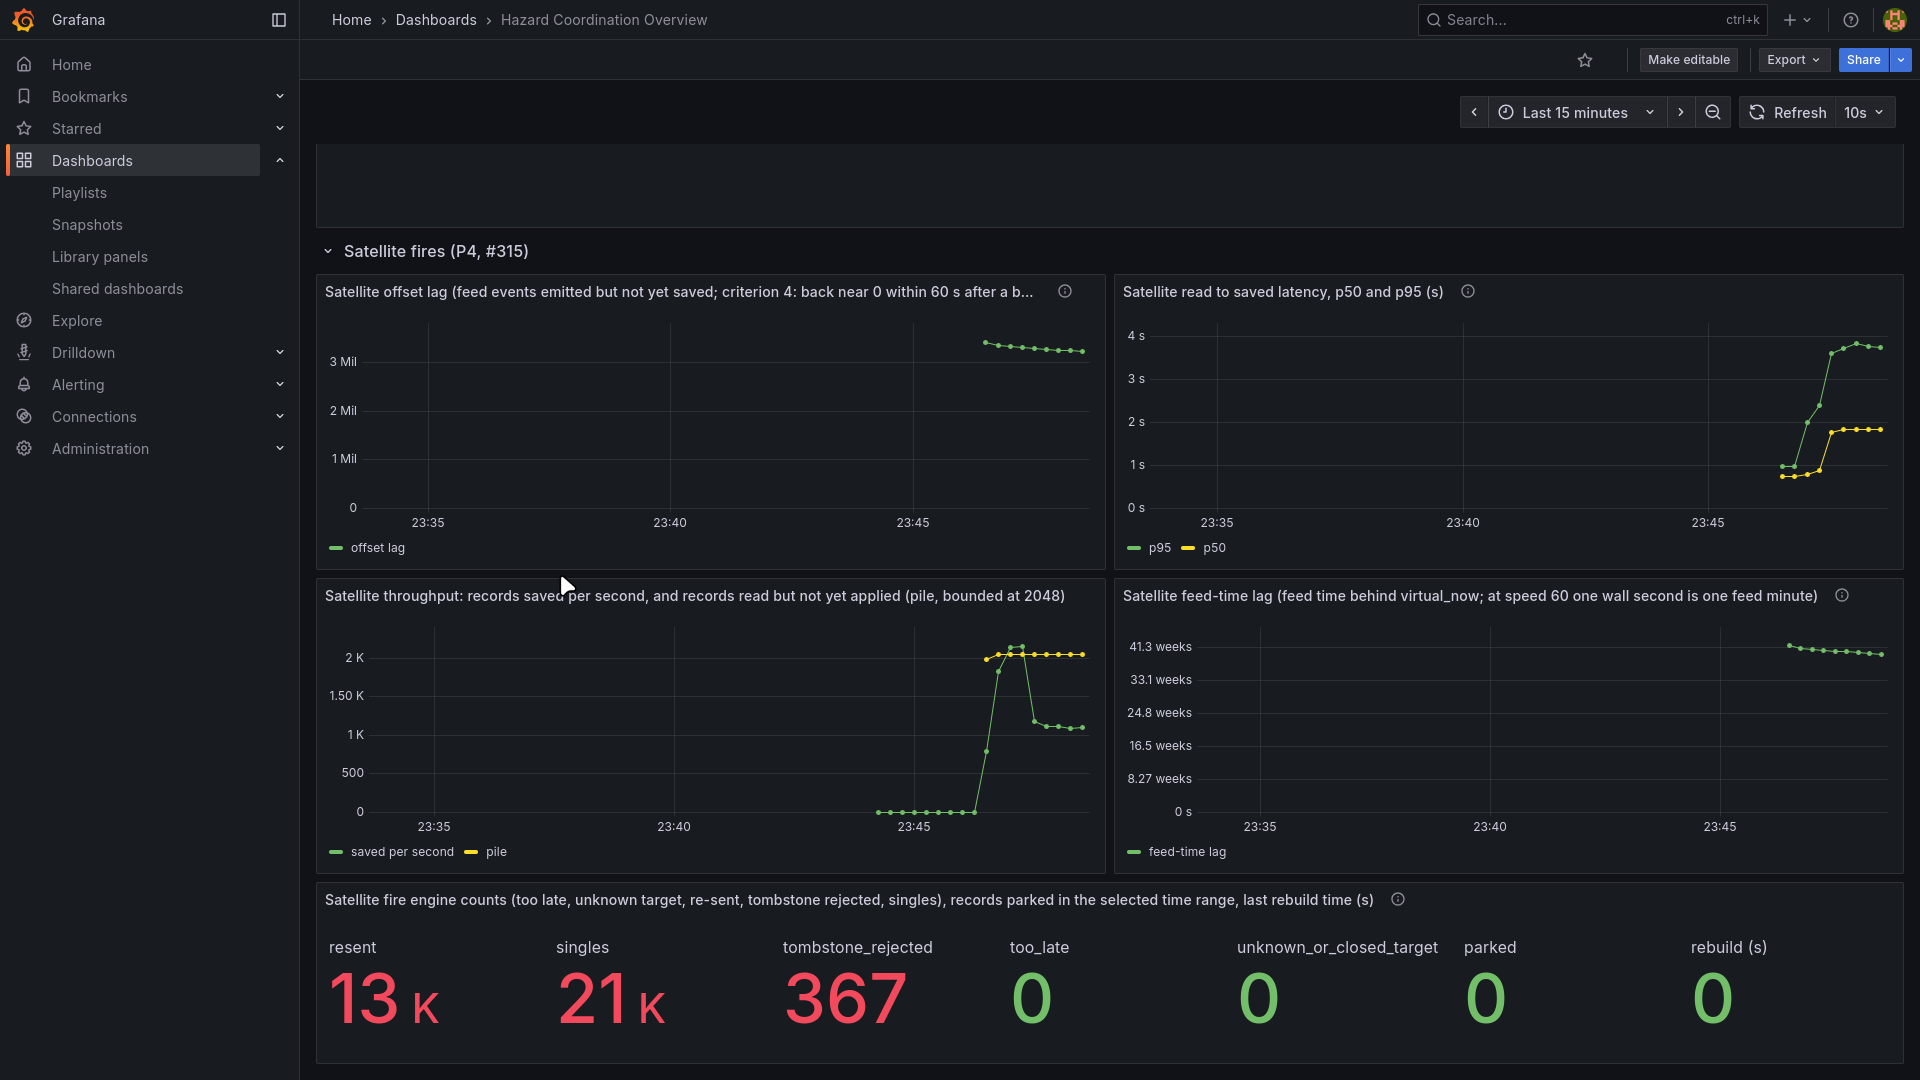
\includegraphics[width=\linewidth,height=0.72\textheight,keepaspectratio]{figures/bukti/p4-grafana-satelit.png}
\caption{Baris \textit{Satellite fires} pada Grafana saat pembacaan ulang}
\label{fig:p4-grafana}
\end{figure}
